\documentclass[a4paper,12pt]{report}

\usepackage{graphicx} 

\begin{document}

\title{Curso práctico multiplataforma de Tratamiento Digital de la Imagen con Jupyter}
\author{ Ana Cuevas Bravo}
\maketitle

\newpage
\pagenumbering{roman}

\renewcommand{\abstractname}{Resumen}
\renewcommand{\chaptername}{Capítulo}
\renewcommand{\chaptername}{Capítulo}

\begin{abstract}
Your abstract goes here...
...
\end{abstract}


\tableofcontents
\newpage
\pagenumbering{arabic}

\chapter{Introducción}
\chapter{Objetivos}
\section{Objetivos}
\section{Requisitos}
\section{Metodología}
\chapter{Infraestructura}

En esta sección se detallan tanto el software empleado para la realización del trabajo, como la estructura previa que existía en la asignatura y que ha servido como base para las nuevas prácticas. \\

 El lenguaje de programación utilizado ha sido Python, profundizaremos en las bibliotecas que tiene este lenguaje para el tratamiento de imagen que han sido necesarias para el desarrollo del trabajo. Esta sección también explicará en que consiste la plataforma Jupyter notebook y las ventajas que tiene en su uso para la docencia. Por último, se hablará de Matlab, la plataforma original que se usa en la asignatura de Tratamiento Digital de la Imagen y la estructura general que tienen las prácticas de esta asignatura.

\section{Python y tratamiento de imagen}

Python es un lenguaje de programación interpretado de alto nivel orientado a objetos creado en los años 80 por Guido van Rossum. Se caracteriza por tener una sintaxis sencilla, fácil de leer, lo que facilita el mantenimiento de programas y lo hace accesible para principiantes. Tiene una amplia biblioteca base y además permite el uso de módulos y paquetes. Al ser interpretado en lugar de compilado el proceso de debugging es más rápido.\\

 Python se está usando cada día más para el tratamiento de imagen, esto se debe a que es un lenguaje muy accesible, siendo gratuito y con una sintaxis sencilla. Con el tiempo han ido surgiendo bibliotecas específicas para el tratameinto de la imagen en Python como Pil (Python Imaging Library) también llamada Pillow, Scikit-image y Open-CV, esta última será la que más se use en este proyecto.\\

Otras bibliotecas que facilitan el tratamiento de imagen en Python son Numpy, una biblioteca para facilitar el uso de matrices y arrays en Python así como las funciones matemáticas relacionadas y Matplotlib que permite  la representación de datos en forma de gráficos.\\

\subsection{OpenCV}

OpenCV(Open Source Computer Vision Library) es una biblioteca centrada en el tratamiento de imagen y video (Computer Vision) y en aprendizaje de máquina, con interfaces para varios lenguajes de programación como C++, Python o Java. OpenCV es la biblioteca de procesamiento de imagen más usada en el mundo con más de 18 millones de descargas. Originalmente programada en C el resto de lenguajes usa diferentes interfaces para acceder al código. Esto permite mejorar el rendimiento siendo C el lenguaje más rápido en ejecución.\\

OpenCV contiene  desde funciones de bajo nivel para el procesado de imagen hasta algoritmos complejos para deteccion de caras. En este trabajo, ya que trata de dar una base de tratamiento de imagen, usaremos funciones de bajo nivel como filtros o funciones para cambiar de espacio de color.\\

Se ha usado la versión 4.2.0 de OpenCV.\\


\subsection{Numpy}

Numpy es el paquete principal para cálculos complejos con matrices en Python, esto lo convierte en un paquete esencial en el desarrollo de código para usos ciéntificos y de robótica. La base de esta biblioteca es el objeto ndarray, que consiste en arrays de n-dimensiones con datos de un mismo tipo y un tamaño establecido al crear la variable, esto último lo diferencia de las listas de python que son dinámicas. Numpy contiene funciones que permiten realizar operaciones con grandes cantidades de datos de una forma más eficiente en memoria y rápida que usando las funciones propias de Python. Numpy está programado y pre-compilado en C. El uso de las funciones de numpy también permite que el código se parezca más a la notación matématica estándar, lo que lo hace más fácil de leer y entender.\\

\subsection{Matplotlib}

Matplotlib es una biblioteca para la creación de gráficos en python. También permite la representacion de imágenes. Matplotlib está construido usando Numpy para funcionar con el paquete general de Scipy. Permite interactúar con los gráficos de una forma muy similar a la representación de Matlab. Matplotlib funciona sobre cualquier sistema operativo. \\

Una de las razones por las que se ha elegido esta biblioteca para representar las diferentes imágenes y gráficos de las prácticas de TDI es por cómo interactúa con los cuadernillos de Jupyter ya que permite la visualización de los gráficos incrustrada en el propio cuadernillo sin crear otra ventana. \\

Otro punto a favor de Matplotlib es la capacidad para interactuar con los gráficos, cómo ya se ha mencionado antes, esto es algo que permite Matlab e interesaba mantener en las prácticas ya que puede ayudar mucho a la hora de entender algunos de los ejercicios. Esta interactividad consiste en la posibilidad de hacer zoom en los gráficos y un cursor que indica el valor del pixel sobre el que está.



\subsection{Scikit-learn}

Esta es una biblioteca con un amplio rango de algoritmos de aprendizaje de máquina para problemas de tamaño medio tanto supervisados como no supervisados.

Scikit-learn está programado mayoritariamente en Python aunque incorpora algunas bibliotecas de C++. Sólo depende de Scipy y Numpy e incorpora código compilado para mejorar su eficiencia.


\section{Jupyter}

El cuadernillo Jupyter es una interfaz web de código libre, que permite la creación de documentos que contienen código ejecutable, ecuaciones, visualización (gráficos, imágenes) y texto.\\
El cuadernillo se guarda como un JSON la extensión .ipnyb. La aplicación es un modelo cliente-servidor que se ejecuta a través de un navegador. Se trata de un servidor local que se crea al ejecutar la aplicación lo que implica que no se necesita conexión a internet para leer o modificar un cuadernillo.  El servidor lee el documento .ipnyb y manda mensajes usando ZeroMQ (una librería que manda mensajes usando un modelo asíncrono) a un kernel que ejecuta el código en el cuadernillo. El cliente funciona en un navegar y es lo que permite interactuar con el cuadernillo.  	\ref{estructurajupyter}
\begin{figure}[h]
\centering
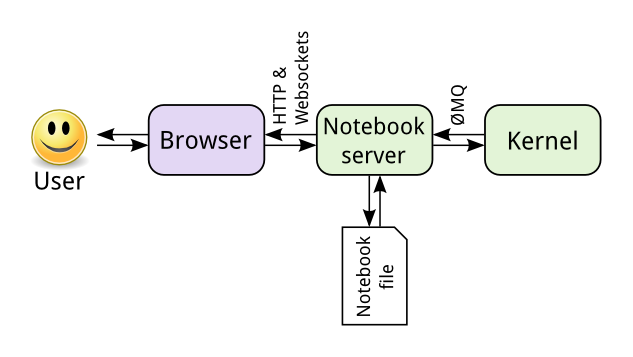
\includegraphics[width=1.0\textwidth]{estructurajupyter}
\caption{estructura de jupyter notebook}
\label{estructurajupyter}
\end{figure}

Los cuadernillos de jupyter consisten principalmente en dos tipos de celdas: code y markdown. Code son las celdas ejecutables en las que se escribe código de python, mientras que markdown son las celdas de texto. Para estilizar el texto se usa  la sintaxis de markdown, que permite desde poner texto en negrita hasta insertar imágenes o fórmulas matemáticas complejas.\\




\section{ Estructura de las Prácticas de TDI en Matlab}


Las prácticas originales para la asignatura de Tratamiento Digital de la Imagen consisten en una carpeta zip que se pone a disposición de los alumnos en el aula virtual de la asignatura. Dentro de esta carpeta están las imágenes que se van a utilizar en la práctica (cuando no eran imágenes internas de MatLab), funciones adicionales necesarias en caso de que no existieran previamente y un enunciado en pdf. En la imagen \ref{carpetapracticas} se puede ver un ejemplo de una de estas carpetas.
 
\begin{figure}[h]
\centering
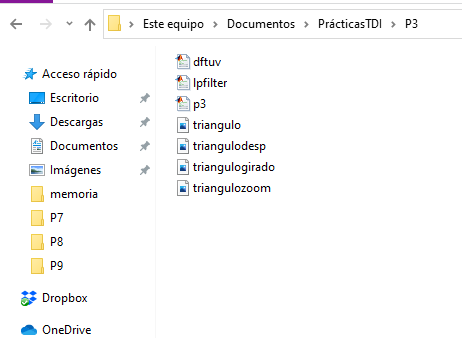
\includegraphics[width=0.5\textwidth]{carpetapracticas}
\caption{ejemplo de carpeta de prácticas}
\label{carpetapracticas}
\end{figure}

Las prácticas se realizaban en hora de clase en uno de los laboratorios de Windows del campus. Se podían realizar enteras en la duración de la clase. \\

La profesora daba una breve explicación inicial sobre el tema de la práctica, siempre relacionado con lo que se hubiera dado en las clases de teoría recientes, el resto de la práctica se podía seguir de forma libre con el enunciado, con la profesora respondiendo las dudas que surgieran en el desarrollo del ejercicio. \\

Los enunciados son instrucciones detalladas sobre los pasos a seguir para realizar la práctica, con poco o nada de teoría, ya que, se asume que el alumno ha recibido las clases de teoría previas. El alumno debe crear un nuevo documento en Matlab e ir ejecutando paso a paso lo que pide el enunciado. \\

Los enunciados suelen comenzar con un breve párrafo explicando el objetivo de la práctica, por ejempl,o en la práctica 4 que trata el tema de segmentación de Imagen la introducción dice: "El objetivo de esta práctica es comenzar a familiarizar al alumno con las herramientas básicas de segmentación de imagen en entorno MATLAB. Para ello se trabajará con la imagen en escala de
grises ‘calculadora.tif’, que acompaña al material de esta práctica. "\\

A partir de esta breve introducción la práctica suele estar dividida en secciones normalmente relacionadas con diferentes puntos tratados en la teoría y como llevarlos a cabo.\\

Los pasos a seguir en MatLab, por lo general, vienen dados en el enunciado que indica qué función usar y cómo llamar a las diferentes variables para mantener una consistencia en los nombres a lo largo de la práctica. En algunos casos se indica las variables necesarias para llamar a la función que se va a usar en esa sección del ejercicio, mientras que en otros se pide al alumno que use el comando \textsl{+help} para informarse sobre el funcionamiento de la función. Del mismo modo si una función requiere de un valor a decidir, dependiendo de lo que se quiera conseguir con su uso, unas veces se da con el enunciado y otras se deja a criterio del alumno para que pruebe como cambian los resultados con diferentes variables y cuál sería la mejor solución para el problema planteado.\\

Otra característica común de los enunciados de TDI son las preguntas para responder, aunque no se pide una memoria en sí de las prácticas en los enunciados hay preguntas con el objetivo de que el alumno se plantee las respuestas y las razones de los pasos que se han ido realizando durante el ejercicio.  La siguiente imagen \ref{preguntasp4} muestra un ejemplo de estas preguntas del principio de la práctica 4.

\begin{figure}[h]
\centering
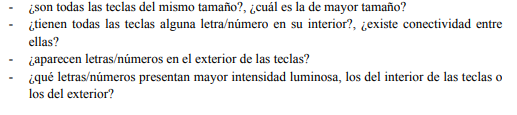
\includegraphics[width=1\textwidth]{preguntasp4}
\caption{ejemplo de preguntas realizadas en los enunciados de TDI}
\label{preguntasp4}
\end{figure}

Algunos de los enunciados tienen imágenes del aspecto que tendría que tener la imagen sobre la que se está trabajando después de ciertos pasos para que el alumno pueda ver si el ejercicio progresa adecuadamente o si debería modificar alguna variable o revisar el código.\\

Si se pide un algoritmo un poco más complejo en los enunciados aparece dado un trozo de ese código como ejemplo o directamente para copiar en matlab ya que el objetivo de estas prácticas no era aprender a programar en MatLab si no ilustrar de forma práctica lo dado en teoría de la asignatura.\\

Las prácticas se suelen centrar en el tratamiento de una imagen en específico, elegida para ilustar el tema del que trata la práctica, por ejemplo en la práctica 1, en el apartado que trata sobre color se escoge una imagen con diferentes verduras que muestran una variedad de colores para ilustrar la mezcla aditiva de color al representarse individualmente las matrices de cada color del sistema de representación RGB. Debido a que algunas de las imágenes usadas en las prácticas originales pertenecen a Matlab o se desconoce su origen se ha tenido que buscar imágenes nuevas, siempre intentando mantener las características de la imagen original.\\

En total la asignatura consiste de 9 prácticas, 7 de imagen y 2 de video. \\

\chapter{Prácticas de TDI}

Este apartado tratará el desarrollo del proyecto, se irá analizando cada práctica de la asignatura y comparando la versión original con el resultado final en python, se tratarán los diferentes porblemas que han ido surgiendo a la hora de adaptar cada práctica y cómo se han solucionado.\\

\section{ Práctica 1: Introducción}

La práctica 1 es una introducción al tratamiento de imagen usando la programación, trata cosas como funciones para representar imágenes, formas de escalar una imagen y manipulación de matrices.\\

\subsection{Teoría tratada en la práctica}

En esta práctica se opera sobre la matriz de la imagen, también se explica de forma práctica la diferencia entre una imagen true color y una imagen indexada. Se pone un énfasis especial en los diferentes tipo de datos en matrices (double, uint64, float...) ya que a la hora de operar puede dar lugar a error.\\

El siguiente punto de la práctica se centra en la conversión de imágenes de color a gris y binario. A continuación se usan diferentes métodos para modificar la resolución de una imagen actuando tanto sobre la resolución espacial como la intensidad.\\

La práctica también explica cómo representar el hitograma de una imagen y el efecto que tiene la ecualización del histograma sobre el conraste de la imagen.\\

Por último se verá la interpretación del color y cómo realizar transformaciones puntuales.\\

\subsection{Comparativa Matlab vs Python}

En este apartado vamos a mencionar las principales diferencias enyre la práctica realizada en Matlab y el nuevo formato usando un cuadernillo de Jupyter.\\

En el primer apartado de la práctica que se centra en la lectura y representación de imágines:\\
La primera diferencia es el espacio de color sobre el que se trabaja. Matlab y matplotlib leen las imágenes de color como RGB mientras que OpenCV usa BGR, esto genera un conflicto entre la librería que se va a usar para leer imágenes y la que se va a usar para representar, se resuelve en el siguiente apartado que trata sobre espacios de color.\\

La segunda diferencia son los métodos de representación, en Matlab teníamos una única funcion (imshow) que crea una ventana nueva con la imagen representada y herramientas como un cursor y la posibilidad de hacer zoom. En pyhton tenemos dos opciones de representación, una es imshow en la biblioteca  OpenCv que al igual que Matlab genera una ventana nueva fuera del cuadernillo pero no tiene herramientas, la otra opción es imshow en Matplotlib que permite visualizar la imagen en el propio cuadernillo y tiene las mismas herramientas que Matlab.
\subsection{Desarrollo de funciones}
\subsection{Resultados}


\section{ Práctica 2: Filtrado espacial}
\subsection{Teoría tratada en la práctica}
\subsection{Comparativa Matlab vs Python}
\subsection{Desarrollo de funciones}
\subsection{Resultados}

\chapter{Conclusiones}

\end{document}